%; whizzy paragraph -pdf xpdf -latex ./whizzypdfptex.sh
%; whizzy-paragraph "^\\\\begin{frame}"
% latex beamer presentation.
% platex, latex-beamer でコンパイルすることを想定。 

%     Tokyo Debian Meeting resources
%     Copyright (C) 2009 Junichi Uekawa
%     Copyright (C) 2009 Nobuhiro Iwamatsu

%     This program is free software; you can redistribute it and/or modify
%     it under the terms of the GNU General Public License as published by
%     the Free Software Foundation; either version 2 of the License, or
%     (at your option) any later version.

%     This program is distributed in the hope that it will be useful,
%     but WITHOUT ANY WARRANTY; without even the implied warreanty of
%     MERCHANTABILITY or FITNESS FOR A PARTICULAR PURPOSE.  See the
%     GNU General Public License for more details.

%     You should have received a copy of the GNU General Public License
%     along with this program; if not, write to the Free Software
%     Foundation, Inc., 51 Franklin St, Fifth Floor, Boston, MA  02110-1301 USA

\documentclass[cjk,dvipdfmx,12pt]{beamer}
\usetheme{Tokyo}
\usepackage{monthlypresentation}

%  preview (shell-command (concat "evince " (replace-regexp-in-string "tex$" "pdf"(buffer-file-name)) "&")) 
%  presentation (shell-command (concat "xpdf -fullscreen " (replace-regexp-in-string "tex$" "pdf"(buffer-file-name)) "&"))
%  presentation (shell-command (concat "evince " (replace-regexp-in-string "tex$" "pdf"(buffer-file-name)) "&"))

%http://www.naney.org/diki/dk/hyperref.html
%日本語EUC系環境の時
\AtBeginDvi{\special{pdf:tounicode EUC-UCS2}}
%シフトJIS系環境の時
%\AtBeginDvi{\special{pdf:tounicode 90ms-RKSJ-UCS2}}

\title{backports.debian.org の活用}
\subtitle{第75回 2011年4月度}
\author{岩松 信洋 iwamatsu@debian.org\\IRC nick: iwamatsu}
\date{2011年4月16日}
\logo{
\includegraphics[width=8cm]{image200607/openlogo-light.eps}}

\begin{document}

\frame{\titlepage{}}

\section{}

\begin{frame}
 \frametitle{アジェンダ}
  \begin{enumerate}
  \item backports.debian.org とは
  \item backports.debian.org で提供されているパッケージを使う
  \item backports.debian.org にパッケージをアップロードする
  \end{enumerate}
\end{frame}

\begin{frame}{backports.debian.orgとは}
\begin{itemize}[<+->]
\item testing や unstable で提供されているパッケージを
既にリリースされた stable および old-stable にバックポートしたパッケージ
を提供するプロジェクト。
\item バックポートされることによって、stable で提
供されているパッケージより新しいバージョンを使うことができるようになる。
\item アップロードされるパッケージには、元のバージョンに\bf{~{}bpo\{Debianリリース番号\}+\{ビルド番号\}}
というバージョンが付加される。
\item セキュリティアップデートにも対応している。\\
DSA(Debian Security Announce)ではなくBSA(Backports Security Announce)
となります。また、DSA とは連動していない点に注意が必要。
\item 2010の9月、正式に debian.org インフラの一部になった。
\end{itemize}
\end{frame}

\begin{frame}[containsverbatim]{backports.debian.orgとは}

\begin{center}
\includegraphics[width=10cm]{image201104/backports-image_color.eps}
\end{center}

\end{frame}

\emtext{backports.debian.org で提供されているパッケージを使う}

\begin{frame}[containsverbatim]{どのようなパッケージが提供されているのか}
\begin{itemize}
\item 現在 backports.debian.org / squeeze-backports で提供されているパッケージは
\url{http://backports.debian.org/changes/squeeze-backports.html}
から参照できる。

\item 既に apt-line に登録している場合には、aptitude で確認できる
\begin{commandline}
$ sudo  aptitude search '?origin(Debian Backports)' -F '%100p'
\end{commandline}

\end{itemize}



\end{frame}

\begin{frame}[containsverbatim]{/etc/apat/sources.list に apt-line を追加する}

/etc/apat/sources.list に backports.debian.org の apt-line を追加する。

squeeze 向けの場合:
\begin{commandline}
deb http://backports.debian.org/debian-backports \
     squeeze-backports main
\end{commandline}

contrib や non-free も提供しているので、有効にしたい場合には apt-line に
追加する。

\end{frame}

\begin{frame}[containsverbatim]

追加したらリポジトリ情報を更新する。

\begin{commandline}
$ sudo apt-get update
または
$ sudo aptitude update
\end{commandline}
\end{frame}

\begin{frame}[containsverbatim]{パッケージをインストールする}

backports.debian.org で提供されているパッケージをインストールするには、
apt や aptitude の \bf{-t} オプションを使って ディストリビューションを指
定する。

postgresql-9.0 パッケージをインストールする場合:
\begin{commandline}
$ sudo apt-get -t squeeze-backports install postgresql-9.0
または
$ sudo aptitude -t squeeze-backports install postgresql-9.0
\end{commandline}

\end{frame}


\begin{frame}[containsverbatim]{パッケージを更新する}

\begin{itemize}
\item backports.debian.org で提供されているパッケージに更新があった場合、
\bf{apt-get update ; apt-get upgrade}を実行しても、パッケージは更新されない。
\begin{itemize}
\item これはPin-Priorityの値が100
(指定すればインストールできるが、アップグレードの対象にはならない)
に設定されているため。
\item 更新するには、apt の preferences を使って、パッケージのプライオリティを設定する必要がある。
\end{itemize}
\end{itemize}

\end{frame}

\begin{frame}[containsverbatim]{パッケージを更新する}

/etc/apt/preferences に以下のような設定をしておくと、
backports.debian.org で提供されているパッケージが更新された場合、
\bf{apt-get update ; apt-get upgrade}で更新されるようになる。

\begin{commandline}
Package: *
Pin: release a=squeeze-backports
Pin-Priority: 200
\end{commandline}

これは、セキュリティアップデートを\bf{apt-get update ; apt-get
 upgrade}で行いたい場合に
必要な設定でもある。


\end{frame}

\begin{frame}[containsverbatim]{Pin-Priorityの値}

常にbackports.debian.org で提供されているパッケージを利用するよう
には、Pin-Priorityの値を500に設定しておくとよい。

Pin-Priority の値と意味(一部):
\begin{table}[ht]
 \begin{center}
  %\caption{Pin-Priority の値と意味}
  \begin{tabular}{|l|p{20em}|}
   \hline
   Pin-Priority & 意味 \\ \hline \hline
   100     & 現在インストールされているパッケージの 優先値\\
   101-500 & 通常のアーカイブよりも優先度が低いが、指定してインストールしたものはアップグレードの対象になる\\
   500     & \bf{ターゲットリリース}に指定されていない通常のアーカイブの優先 \\
   \hline
  \end{tabular}
 \end{center}
\end{table}

\end{frame}

\begin{frame}[containsverbatim]{セキュリティアップデート}
\begin{itemize}
\item backports.debian.org で提供されているパッケージのセキュリティアップデー
トは DSA では行われない。
\item BSAとして行われ、 誰かがアップロードを行う。

(backports チームが監視していると思われる。)

\item パッケージアップデートのアナウンスは
backports-announce メーリングリスト
(\url{http://lists.debian.org/debian-backports-announce})
で行われる。

backports.debian.orgを使っている人はメーリングリストに登録
しましょう。
\end{itemize}

\end{frame}


\begin{frame}[containsverbatim]{バグレポート}
\begin{itemize}
\item 今のところ、backports.debian.org で提供されているパッケージは Debian
BTS(\url{http://bugs.debian.org}) にバグレポートしてはいけないことになっ
      ている。
\item なにか問題があった場合には、backports メーリングリスト(\url{http://lists.debian.org/debian-backports})
に投稿する。

\item backports.debian.org は Debian の正式なインフラなので、Debian BTS
      に統合される可能性もある。
その場合には、reportbug パッケージからもバグレポートできるようになるかも
しれない。
\end{itemize}

\end{frame}


\begin{frame}{欲しいパッケージがない場合}

自分の欲しい機能がまだ stable で提供されているパッケージにない!
しかし、unstable にあるパッケージにはあるようだ。どうすればいい?


\begin{itemize}[<+->]
\item 自分でビルドして使う。
\item \sout{2ch に書く。}
\item debian-users@l.d.o.j に相談する。
\item パッケージメンテナに相談する。
\item backports.debian.org で提供してもらうように依頼する。
(\url{http://lists.debian.org/debian-backports/})
\end{itemize}

\end{frame}

\emtext{backports.debian.org を使ったパッケージの提供方法}

\begin{frame}[containsverbatim]{backports.debian.org を使ったパッケージの提供方法} 

\begin{itemize}
\item backports.debian.org は誰でも利用可能。
\item パッケージをアップロードするには、Debian Developer(以下、DD)であ
      る必要がある。
\item Debian Maintainer もパッケージをアップロードおよび更新はできない。
\item DD以外はスポンサーアップロードをしてもらう必要がある。
\item 自分がメンテナンスしているパッケージ以外でもアップロードできる。
\end{itemize}

\end{frame}

\begin{frame}[containsverbatim]{backports.debian.org キーリングへの登録}

\begin{itemize}
\item DDでもすぐにアップロードできるわけではない。
\item Debian Developer キーリングと同じ鍵を backports.debian.org キーリ
      ングへの登録してもらう必要がある。
\item 申請はリクエストトラッカー
(\url{https://rt.debian.org/Ticket/Create.html?Queue=20})を使って行う。

\item 申請すると、数日後にキーリングに追加される。
\end{itemize}

\end{frame}


\begin{frame}[containsverbatim]{アップロードするパッケージについて}

\begin{itemize}
\item backports.debian.org にアップロードするパッケージは
 testing や unstable にあるパッケージをリビルドしてアップロードするのでは
なく、パッケージそのものに手を加える必要がある。
\item 注意する点もいくつかある。
\end{itemize}

\end{frame}




\begin{frame}[containsverbatim]{ディストリビューションを コードネーム-backports に変更する}

\begin{itemize}
\item debian/changelog では、ディストリビューションに stable 
や unstable を設定しますが、backports.debian.org にアップロードするパッ
ケージのディストリビューションには \bf{コードネーム-backports} を指定す
      る必要がある。
例えば、squeeze へバックポートしたい場合には、\bf{squeeze-backports}とす
      る。
\end{itemize}

\end{frame}


\begin{frame}[containsverbatim]{Debian バージョンに\bf{~{}bpo\{Debianリリース番号\}+\{ビルド番号\}}を付加する}

\begin{itemize}
\item backports.debian.org にアップロードされるパッケー
ジには他のディストリビューションとの違いが分かるようにDebian バージョン
に\bf{~{}bpo\{Debianリリース番号\}+\{ビルド番号\}}というバージョンを付
加する必要がある。
\item unstable にある パッケージ foo の \bf{1.2.3-4} をアップロードし
squeeze-backports にアップロードしたい場合には、\bf{1.2.3-4~{}bpo60+1}
とする。60は squeeze のリリース番号(6.0)。
\item アップロードしたパッケージ問題があり、再アップロードしたい場合には、
\bf{1.2.3-4~{}bpo60+2}とし、ビルド番号をインクリメントする。
\end{itemize}

\end{frame}

\begin{frame}[containsverbatim]
\begin{commandline}
  1 bluez (4.91-1~bpo60+1) unstable; urgency=low
  2 
  3   * Rebuild for squeeze-backports.
  4 
  5  -- Nobuhiro Iwamatsu <iwamatsu@debian.org>  Sat, 16 Apr 2011 03:31:07 +0900
  6 
  7 bluez (4.91-1) unstable; urgency=low
  8 
  9   * New upstream release.
\end{commandline}

\end{frame}



\begin{frame}[containsverbatim]{backports だけの修正を行わない}
\begin{itemize}
\item 特定のバージョンで発生するのはバグなので、unstable 等で修正して、それを
backports.debian.org にバックポートする。
\end{itemize}

\end{frame}


\begin{frame}[containsverbatim]{squeezeおよびbackportsの環境でパッケージがビルドできるか確認する}
\begin{itemize}
\item backports.debian.org では、buildd と同様に複数のアーキテクチャ向けにパッ
ケージがビルドされる。
\item stableおよびbackportsの環境でパッケー
ジがビルドできない場合、FTBFS(Fail To Build From Source)になるため、
注意が必要。
\item ABIの問題があるため、動作確認は慎重に行う必要があ
ります。

\item pbuilder\footnote{http://packages.qa.debian.org/p/pbuilder.html}
や cowbuilder\footnote{http://packages.qa.debian.org/c/cowdancer.html} を使っ
て、クリーンルームからのビルドチェッ
クを行う。
\item バックポートに足りないパッケージがあるようなら、そのパッケージもバッ
      クポートする事。
\end{itemize}

\end{frame}

\begin{frame}[containsverbatim]{インストールとアップデートの確認をする}
\begin{itemize}
\item パッケージができても、インストールとアップデートがうまく動作しない場合が
 ある。
\item これは、
piuparts\footnote{http://packages.qa.debian.org/p/piuparts.html}
を使って確認できる。
\end{itemize}

\end{frame}


\begin{frame}[containsverbatim]{パッケージのアップロード先}
\begin{itemize}
\item 通常、パッケージは\url{ftp.upload.debian.org}にアップロードされる。
\item backports.debian.orgの場合には、
\url{backports-master.debian.org}にアップロードする必要がある。
\item アップロードする前に、dput や dupload 
の設定ファイルにbackports.debian.org向けの設定を加えておく。
\end{itemize}


\end{frame}

\begin{frame}[containsverbatim]

\begin{itemize}
\item dupload の場合
\begin{commandline}
$cfg{'bpo'} = {
  fqdn => ``backports-master.debian.org'',
  incoming => ``/pub/UploadQueue/'',
};
\end{commandline}

\item dput の場合
\begin{commandline}
[bpo]
fqdn = backports-master.debian.org
incoming = /pub/UploadQueue/
method = ftp
login = anonymous
allow_dcut = 1
\end{commandline}
\end{itemize}

\end{frame}

\begin{frame}[containsverbatim]{セキュリティアップロードをする}
\begin{itemize}
\item backports-master.debian.org にセキュリティアップロードを行う場合には
BSA 番号を割り振ってもらう必要がある。
\item この番号は backports チームで管理しているので、
      \url{team@backports.debian.org}に問い合わせる事。
\item セキュリティアップロードの内容をPGP/GPGでサインして、
backports-announce メーリングリスト
      (http://lists.debian.org/debian-backports-announce)にアナウンス
      する。
\end{itemize}
\end{frame}

\begin{frame}[containsverbatim]{backports.debian.org の動作}
backports.debian.org の動作は buildd network と同じ。
アップロード先やパッケージリポジトリが異なるだけで、buildd networkを
利用したパッケージのビルドを行っている。

\begin{center}
\includegraphics[width=10cm]{image201104/backports-buildd_color.eps}
\end{center}
\end{frame}

\emtext{まとめ}
\begin{frame}[containsverbatim]{まとめ}
\begin{itemize}
\item ユーザが backports.debian.org を使う場合、新しいバージョンを使えるという
メリットがあるので使ったほうが良い。
\item BTS等はうまく連動していないのと、パッケージメンテナでは
なくてもアップロードできてしまうので、問題があった場合には調整が必要にな
ることがあるかも。
\item このような場合には debian-backports メーリングリス
トをうまく活用していく必要がある。
\item apt の pin の設定を正しくしておかないと、うまくアップデートしなかっ
たりするので、注意が必要。

\item 開発者の場合には、メンテナンスコストが増えるだけであまりメリットがあるよ
うには思えない(個人的に)。
\item しかしユーザからの依頼があった場合には考慮する必要が
あるので、仕組みだけは知っておくとよいかも。
\item もう少し使いやすくするには他のDebianインフラとの連携が密になる必要
      があると思う。
\end{itemize}

\end{frame}

\end{document}
